\subsection{Event channel and decoupling}
\label{sec:eventchannel}
One of the design goals is robustness of the framework facilities,
and SWIM decouples utilities as much as possible. The main mechanism is using
an ``event channel'', a daemon service running at a well-known location.
Even different portlets running within the same portal try to use the event
channel whenever possible, instead of internal portal mechanisms.

The SWIM project uses the WS-Messenger (WSMG) \cite{wsmg,wsmgpaper} web service,
developed by the Extreme Lab at Indiana University, as an
event channel. Supporting both 
the WS-Eventing and WS-Notification specifications, WSMG is a
publish-subscribe system that allows
components or portal utilities to publish notifications
about events that occur during a run of a code.  A notification
consists of a message and a topic.  To receive notifications, a
utility must subscribe to a specific topic.  This is a
many-to-many relationship, as a subscriber can subscribe to many
different topics and a publisher's notifications may be consumed
by many different subscribers.

Using a publish-subscribe event channel like WSMG allows us to
decouple the event handling from the actual running of codes.
WSMG runs on a separate ``broker'' machine and maintains a
database of current subscriptions.  Publishers send events
consisting of a message and a topic to the broker, which then
sends the events to all subscribers interested in that particular
topic.  The publisher does not need to know which, if any,
subscribers are receiving its events.

WS-Messenger is currently being used in the Linked Environments
for Atmostpheric Discovery (LEAD)\cite{lead} project to allow remote
applications to send notification messages to each other.

\begin{figure}
\centering
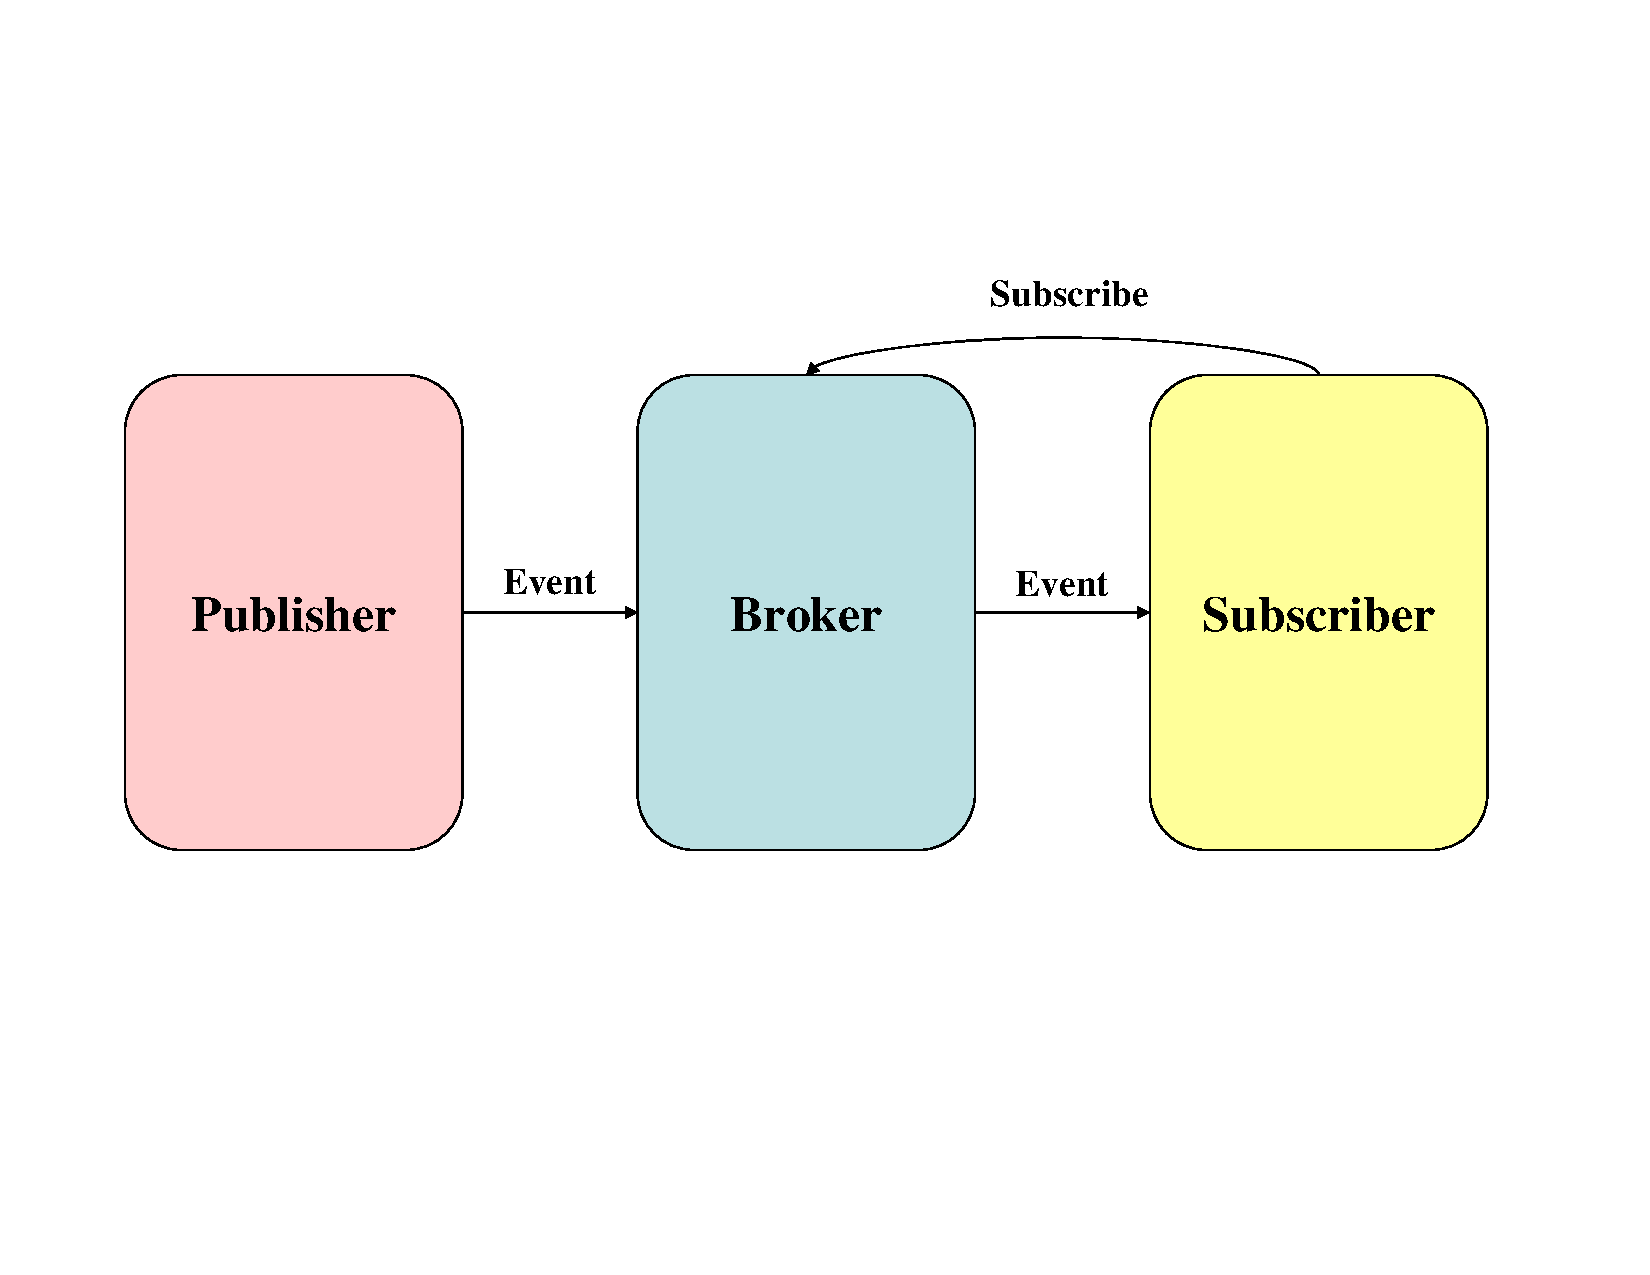
\includegraphics[width=3.0in]{eventpic}
\caption{Event Channel}
\label{eventchannelpic}
\end{figure}

